\documentclass{beamer}
\usepackage[utf8]{inputenc}
\usepackage{listings}
\usepackage{booktabs}
\usepackage{amssymb}
\usepackage{nicefrac}
\usepackage{amsmath}
\usepackage{bbm}
\usepackage{bm}
\usepackage{enumitem}
\usepackage{hyperref}
\usepackage[export]{adjustbox}
\usepackage{svg}

\usetheme{Madrid}
\definecolor{mlpblue}{rgb}{0.1, 0.14, 0.24}

\useoutertheme{infolines} % Alternatively: miniframes, infolines, split
\useinnertheme{circles}
\usecolortheme[named=mlpblue]{structure}

\DeclareMathOperator{\Tr}{Tr}
\DeclareMathOperator{\Cov}{Cov}
\DeclareMathOperator{\Concat}{Concat}

\DeclareMathOperator*{\argmax}{arg\,max}
\DeclareMathOperator*{\argmin}{arg\,min}
\DeclareMathOperator*{\indep}{\perp \!\!\! \perp}

\lstset{basicstyle=\footnotesize\ttfamily,breaklines=true}

%------------------------------------------------------------
%This block of code defines the information to appear in the
%Title page
\title[Cosmos ]{World Foundation Model Platform for Physical AI}

\subtitle{Cosmos} %\thanks{Beaglehole, Súkeník et.~al.~[NeurIPS 2024]}}
\author[MLP]{A. Buynitsky} 
\date{Jan 28, 2025}
\titlegraphic{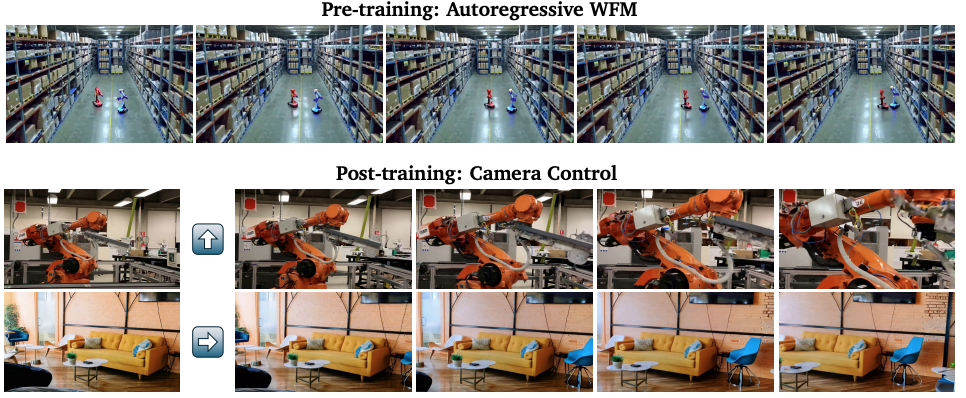
\includegraphics[width=8cm]{./img/title.png}}

%End of title page configuration block
%------------------------------------------------------------

%The next block of commands puts the table of contents at the 
%beginning of each section and highlights the current section:

\AtBeginSection[]
{
  \begin{frame}
    \frametitle{Outline}
    \tableofcontents[currentsection]
  \end{frame}
}
% ------------------------------------------------------------


\begin{document}

\frame{\titlepage}


%---------------------------------------------------------
% This block of code is for the table of contents after
% the title page
\begin{frame}
\frametitle{Outline}
\tableofcontents
\end{frame}
%---------------------------------------------------------
\section{TLDR}
\begin{frame}[t]{TLDR (part 1)}
    \textbf{Problem:} More efficient to train agents virtually which requires virtual platforms \newline
    \textbf{Solution:} World Foundation Models (WFMs) that can be pretrained and finetuned similar to LLMs\newline
    \begin{center}
        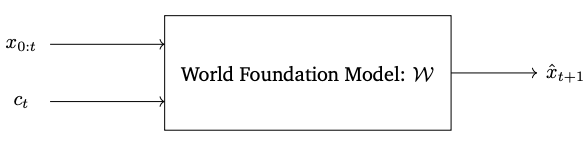
\includegraphics[width=0.8\textwidth]{./img/tldr_2.png}
    \end{center}
    \textbf{WFM Goal}: predict future observation $\hat{x}_{t+1}$ based on $ x_{0:t}$ and $c_t$
    \small
    \begin{itemize}[label=-]
        \item $ x_{0:t}$ sequence of $t$ timesteps of visual observed data
        \item $c_t$ takes on many forms (actions, trajectories, text descriptions)
        \item $ x_{0:t}$ sequence of $t$ timesteps of visual observed data
    \end{itemize}
    \normalsize
            
\end{frame}

\begin{frame}[t]{TLDR (part 2)}
    \textbf{Problem:} More efficient to train agents virtually which requires virtual platforms \newline
    \textbf{Solution:} World Foundation Models (WFMs) that can be pretrained and finetuned similar to LLMs\newline
    \textbf{Results:} 
    \begin{center}
        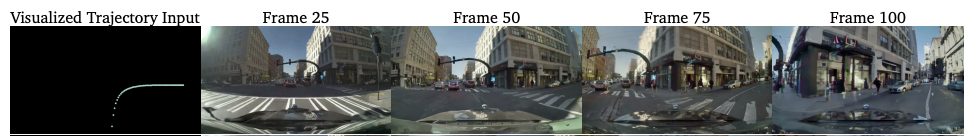
\includegraphics[width=\textwidth]{./img/tldr_1.png}
    \end{center} 
    \textbf{Research Group:} NVIDIA + 1X\newline
    \textbf{Future Work:}
    \small
    \begin{itemize}[label=-]
        \item \textbf{Policy Evaluation:} benchmarking policies in simulator vs real-world
        \item \textbf{Policy Initialization:} well-trained WFM can initialize policies 
        \item \textbf{Policy Training:} WFM pairmed with reward can give feedback in RL
        \item \textbf{MPC Control:} WFM predict future sttates of physical system
    \end{itemize}
    \normalsize
\end{frame}


\begin{frame}[t]{TLDR (part 3)}
    \begin{center}
        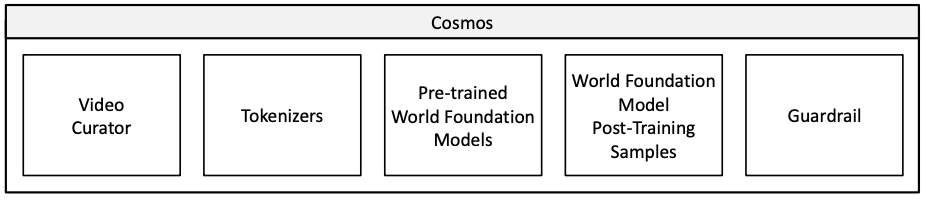
\includegraphics[width=\textwidth]{./img/tldr_3.png}
    \end{center} 
    \small
    \begin{itemize}[label=-]
        \item \textbf{Video Currator:} Collecting high-quality pre-training data
        \item \textbf{Tokenizers:} Image and video tokenizers
        \item \textbf{Pre-trained WFMs:} Diffusion and Autoregressive models
        % text2world generation pre-training
        % video2world generation pre-training
        \item \textbf{WFMs Post-Training:} finetuning for specific robotic tasks
        \item \textbf{Guardrail:} safety to block harmful input and outputs
    \end{itemize}
    \normalsize
\end{frame}


\section{Data Curation}

\begin{frame}[t]{Raw Data}
    Collect 20M hours of videos from a diverse set of physical AI environments
    \begin{columns}
        \hspace{1em}
		\begin{column}{.5\textwidth}
            \small
            \begin{enumerate}[label=\arabic*., itemsep=0.5mm]
                \item Driving (11\%)
                \item Hand motion and object manipulation (16\%)
                \item Human motion and activity (10\%)
                \item Spatial awareness and navigation (16\%)
                \item First person point-of-view (8\%)
                \item Nature dynamics (20\%)
                \item Dynamic camera movements (8\%)
                \item Synthetically rendered (4\%)
                \item Others (7\%)
            \end{enumerate}
            \normalsize
		\end{column}
        \hspace{0em}
		\begin{column}{.5\textwidth}
            \textbf{Problem:} redundant / useless information \newline
            \textbf{Solution:} Filtering / Postprocessing \newline
            \textbf{Result:} $10^8$ pre-training video clips and $10^7$ finetuning clips 

		\end{column}
        \hspace{2em}
	\end{columns}
\end{frame}

% \item train to minimize: \[\mathcal{L}_{NLL} = \sum_i -log \pi_\Theta(v_i | v_1, v_2, \dots, v_{i-1})\]begin{frame}[t]{Splitting}
%     \textbf{Problem:} Videos have arbitrary lenghts and might contain shot transitions
%     % ex: two ppl talking in kitchen in NYC to lions in savana
%     % important to segment videos base on shot chagnes and generate consistent video clips physically plausible
%     \textbf{Shot Detection}
%     \begin{itemize}[label=-]
%         \item Generate start and end frame indices of clips using TransNetV2
%         \item Discard clips shorter than 2s, slipt clips over 60s long % (visual effects / transitions)
%         % create own internal benchmark, TransNetV2
%         % Normalize all videos to the same codec 
%     \end{itemize}
%     \textbf{Filtering} % remove clips with bad quality, select high-quality for fine-tuning, tailor data distrubtion for MFs
%     \begin{itemize}[label=-]
%         \item \textbf{Motion Filtering:} remove static videos / with abrupt camera motion / tag videos with differnet camera motion 
%         % create own internal benchmark, TransNetV2
%     \end{itemize}
% \end{frame}


\section{Tokenizer}
\begin{frame}[t]{Tokenizers}
    Visual tokenizers map raw visual data (images, videos) to compact tokens
        \begin{center}
            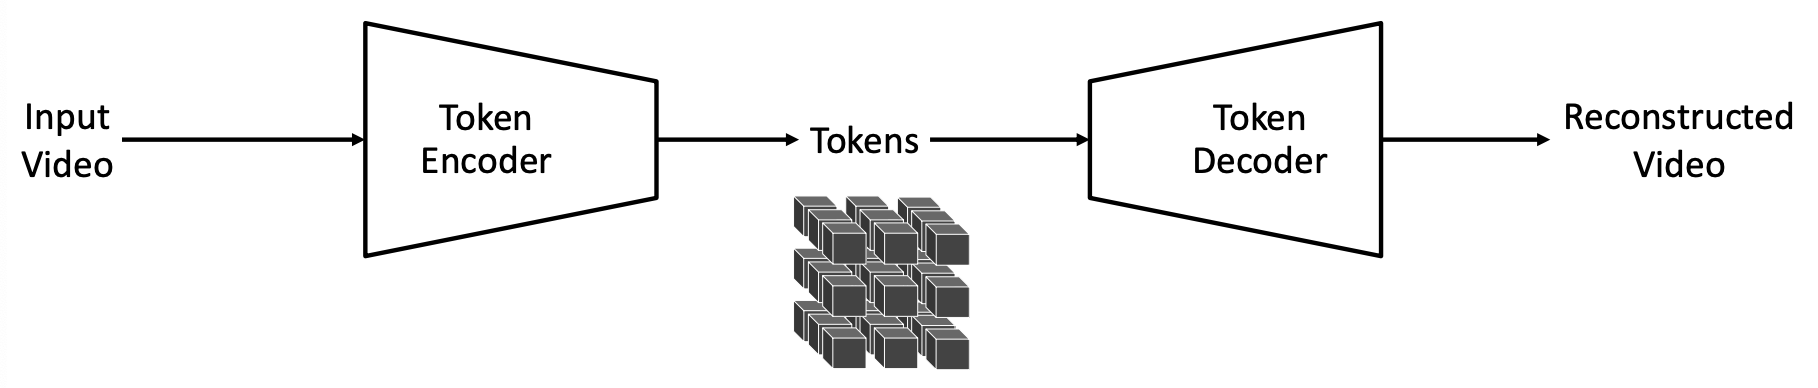
\includegraphics[width=0.8\textwidth]{./img/tokenizer_1.png}
        \end{center}
	\begin{columns}[t]
		\begin{column}{.5\textwidth}
            \textbf{Continuous Tokenizers:} Encode into continuous latent embeddings \newline
            % cont tokenizers: a set of vectors as in stable diffusion
            \vspace{-1.5em}
			\begin{center}
                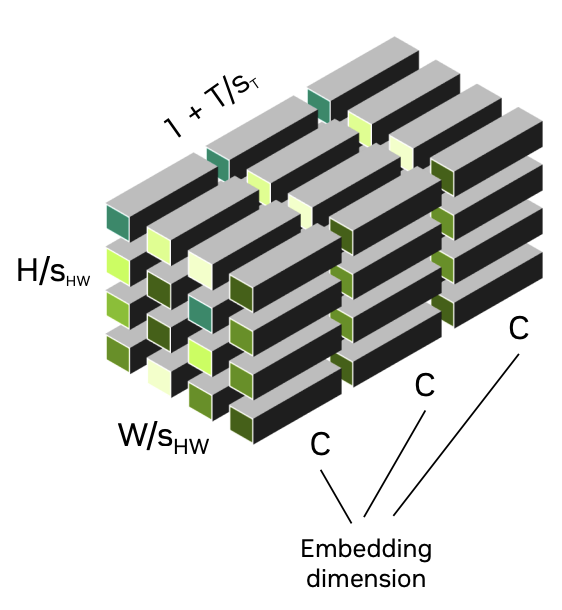
\includegraphics[width=0.5\textwidth]{./img/tokenizer_cont.png}
			\end{center}
		\end{column}
		\begin{column}{.5\textwidth}
            \textbf{Discrete Tokenizers:} Encode into discrete latent codes
            % disc tokenizers: make to quantized indices ie autoregressive transformers GPT
            % trade off between high compression rates without compromizing subsequent visual reconstruction quality
            % high comperssing reduces storage / computation
            % excessvie compression lead to loss of details
            \vspace{-0.5em}
			\begin{center}
                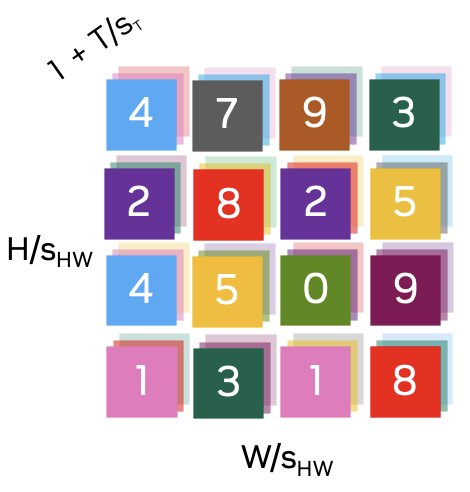
\includegraphics[width=0.5\textwidth]{./img/tokenizer_discrete.png}
			\end{center}
		\end{column}
	\end{columns}
    % 1 + just to not have 0
    $S_{HW}$: Spatial compression factor, $S_T$: Temporal compression factor
\end{frame}

\begin{frame}[t]{Cosmos Tokenizer}
    Encoder Decoder Architecture: given $x_{0:T} \in R^{(1+T) \times H \times W \times 3}$
        \begin{gather}\label{eq:1}
            \varepsilon(x_{0:T}) = z_{0:T'} \in \mathbb{R}^{(1+T') \times H' \times W' \times C'}  \\
            \mathcal{D}(z_{0:T'}) = \hat{x}_{0:T} \in R^{(1+T) \times H \times W \times 3}
        \end{gather}
	\begin{columns}[t]
		\begin{column}{.5\textwidth}
            \textbf{Continuous Tokenizers:} Encode into continuous latent embeddings \newline
            % cont tokenizers: a set of vectors as in stable diffusion
            \vspace{-1.5em}
			\begin{center}
                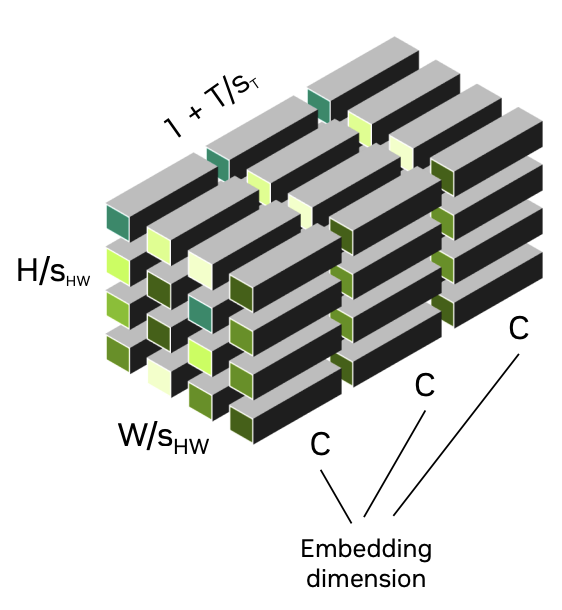
\includegraphics[width=0.5\textwidth]{./img/tokenizer_cont.png}
			\end{center}
		\end{column}
		\begin{column}{.5\textwidth}
            \textbf{Discrete Tokenizers:} Encode into discrete latent codes
            % disc tokenizers: make to quantized indices ie autoregressive transformers GPT
            % trade off between high compression rates without compromizing subsequent visual reconstruction quality
            % high comperssing reduces storage / computation
            % excessvie compression lead to loss of details
            \vspace{-0.5em}
			\begin{center}
                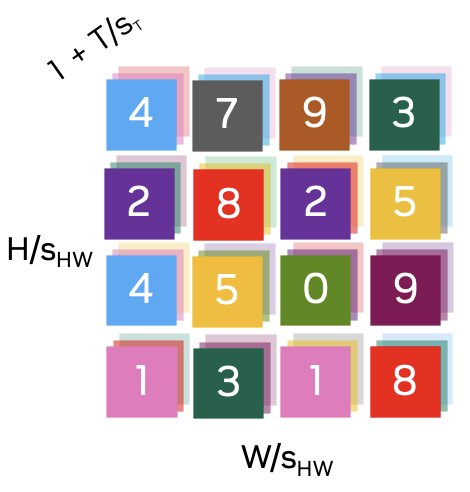
\includegraphics[width=0.5\textwidth]{./img/tokenizer_discrete.png}
			\end{center}
		\end{column}
	\end{columns}
    % 1 + just to not have 0
    $S_{HW}$: Spatial compression factor, $S_T$: Temporal compression factor
\end{frame}

\begin{frame}[t]{Cosmos Tokenizer}
    \vspace{-2em}
	\begin{columns}[t]
		\begin{column}{.5\textwidth}
            \begin{center}
                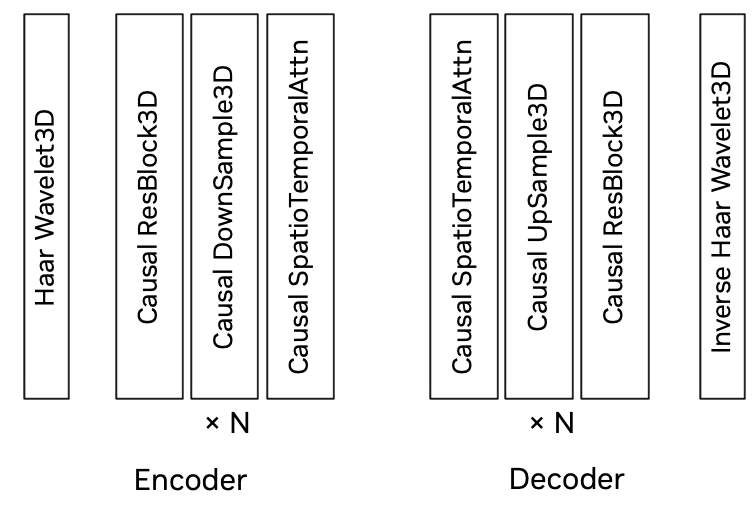
\includegraphics[width=0.8\textwidth]{./img/tokenizer_2.png}
            \end{center}
		\end{column}
		\begin{column}{.5\textwidth}
            \begin{center}
                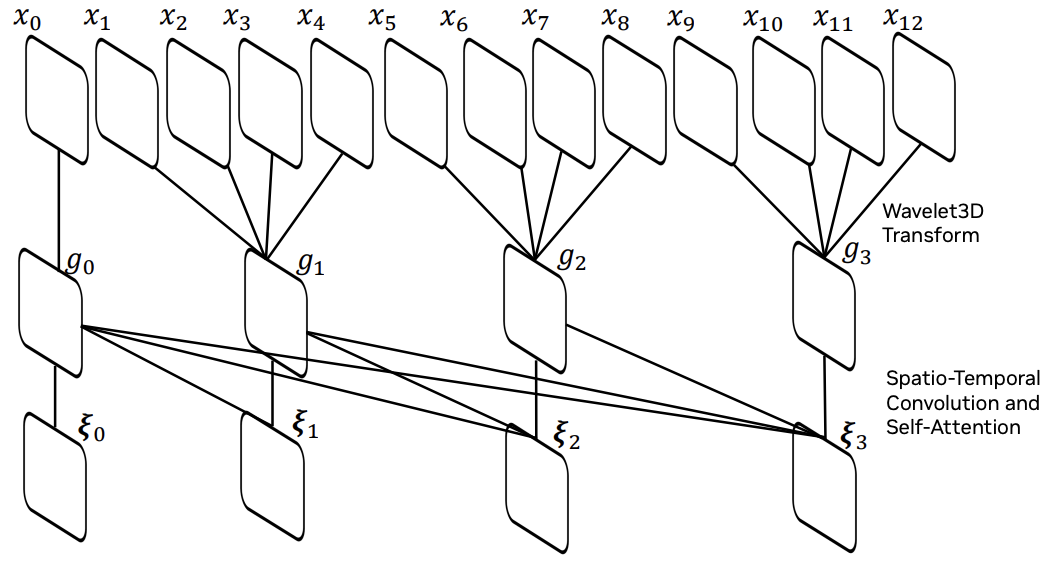
\includegraphics[width=0.8\textwidth]{./img/tokenizer_3.png}
            \end{center}
		\end{column}
	\end{columns}
    \small
\end{frame}

\begin{frame}[t]{Wavelet Transform}
    \textbf{Wavelet:} compress long signals into smaller ones
    \[
    \text{Let } W = 
    \left
    \{
    \begin{vmatrix}
      1 \\
      1 \\
      1 \\
      1 
    \end{vmatrix}
    ,
    \begin{vmatrix}
      1 \\
      1 \\
     -1 \\
     -1 
    \end{vmatrix}
    ,
    \begin{vmatrix}
      1 \\
     -1 \\
      0 \\
      0
    \end{vmatrix}
    ,
    \begin{vmatrix}
      0 \\
      0 \\
      1 \\
     -1
    \end{vmatrix}
    \right
    \}
    \text{be the Haar basis}
    \]
    \[
    E = \left\{e_1, e_2, e_3, e_4 \right\} \text{be standard basis of }  \mathbb{R}^4
    \]
    \normalsize
    (pairwise orthogonal vectors are linearly independent)\newline
    The change of basis matrix from $W$ to $E$, $T_{W,E}$ is given by:
    \[T_{W,E} = 
        \begin{vmatrix}
            1 & 1 & 1 & 0 \\
            1 & 1 & -1 & 0\\
            1 & -1 & 0 & 1\\
            1 & -1 & 0 & -1 
          \end{vmatrix}
    \]
\end{frame} 


\begin{frame}[t]{Wavelet Transform}
    Given a signal $v =\begin{vmatrix} v_1 & v_2 & v_3 & v_4 \end{vmatrix}^T$, transform 
    $v$ into its coefficients over the Haar Basis by computing $c=\begin{vmatrix} c_1 & c_2 & c_3 & c_4 \end{vmatrix}^T= T_{W,E}^{-1} v$ \newline

    \textbf{Example:}
    Take $v = \begin{vmatrix} 6 & 4 & 5 & 1 \end{vmatrix} $ over the basis $E$
    \[c= T_{W,E}^{-1} \cdot v = \begin{vmatrix} 4 & 1 & 1 & 2 \end{vmatrix}\] 
    Observe that: $c_1 =\frac{v_1 + v_2 + v_3 + v_4}{4}$ is the average value of signal $v$ %correspond to background of the image.
    \newline
    $c_2$ gives coarse details of $v$ \newline 
    $c_3$ gives details in first part of $v$ \newline
    $c_4$ gives details in second part of $v$ \newline
    Reconstruct signal by $v = T_{W,E} \cdot c$ \newline
    \newline
    \textbf{Compression:} Throw away some of coefficients of $c$ (settinig them to zero)
    \newline
    Cosmos Tokenizer does two stages of compression, reducing resultion of $x$, $y$ and $t$ by half in each (4x reduction total)\newline
\end{frame} 

\begin{frame}[t]{Cosmos Tokenizer}
    \vspace{-2em}
	\begin{columns}[t]
		\begin{column}{.5\textwidth}
            \begin{center}
                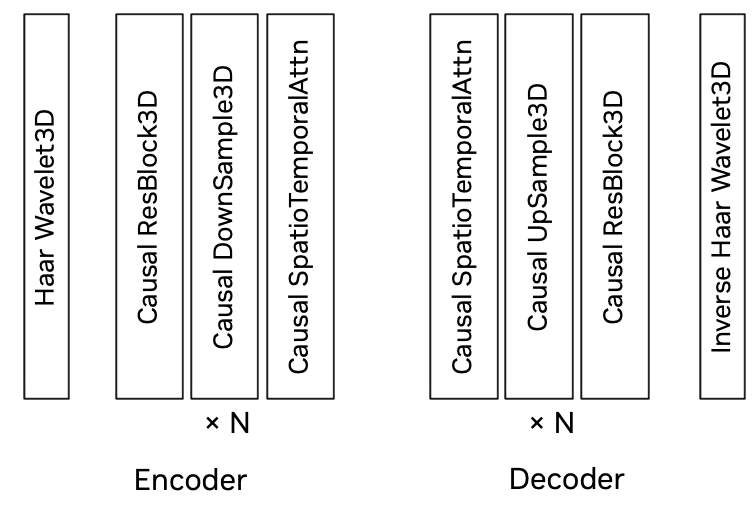
\includegraphics[width=0.8\textwidth]{./img/tokenizer_2.png}
            \end{center}
		\end{column}
		\begin{column}{.5\textwidth}
            \begin{center}
                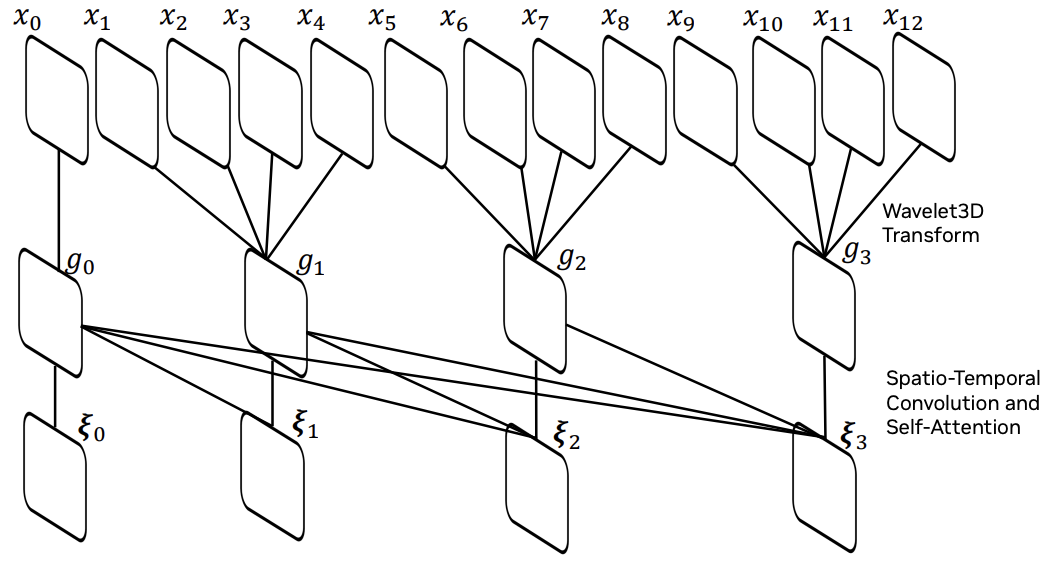
\includegraphics[width=0.8\textwidth]{./img/tokenizer_3.png}
            \end{center}
		\end{column}
	\end{columns}
    \textbf{Downsampling}
    \begin{itemize}[label=-]
        \item 2D convolution with kernel $1 \times k \times k$ for spatial info 
        \item 1D convolution with kernel $k \times 1 \times 1$ for temporal info (left padded with $k-1$)
        \item spatio-temporal attention (ie. $1 + T'$ for last encoder block)
        % spatio-temoral attention: at time i, only attend from 0:i
    \end{itemize}
    \textbf{Continuous:} Use vanilla Autoencoder for latent space (dim = 16)
    \textbf{Discrete:} project using Finite-Scalar-Quantization to 64k vocab size
    % FSQ: small dimension (they used 6), and each dimension is quantized to small set of fixed values
\end{frame}

\begin{frame}[t]{Cosmos Tokenizer Training}
    Supervise the final output of tokenizer's decoder (no aux loss ie KL), train by alternating images and videos \newline
    \textbf{Stage 1:}
    \[\mathcal{L}_1 = \| \hat{x}_{0:T} - x_{0:T} \|_1\]
    % xhat is reconstructed image
    \[\mathcal{L}_{\text{Perceptual}} = \frac{1}{L} \sum_{l=1}^{L} \sum_{t} \alpha_l \| \text{VGG}_l(\hat{x}_t) - \text{VGG}_l(x_t) \|_1\]
    % vgg  alpha: predefined weights
    \textbf{Stage 2:} \newline
    % optical flow: how objects movethrough video 
    \textbf{Optical Flow loss} for temporal smoothness
    \[\mathcal{L}_{\text{Flow}} = \frac{1}{T} \sum_{t=1}^{T} \| \text{OF}(\hat{x}_t, \hat{x}_{t-1}) - \text{OF}(x_t, x_{t-1}) \|_1\]    
    \textbf{Gram-matrix loss} for sharpness of reconstructed images
    \[\mathcal{L}_{\text{Gram}} = \frac{1}{L} \sum_{l=1}^{L} \sum_{t} \alpha_l \| \text{GM}_l(\hat{x}_t) - \text{GM}_l(x_t) \|_1\]
\end{frame}
% results: faster / better than other tokenizers for video data, 2x -12x faster
% have a spatila compression of 4 x 8 x 8 is best, even lower, 8 x 8 x 4 or 8 x 16 x16, have comparable perf
\section{Diffusion-based WFM}

\begin{frame}[t]{Formulation}
    \textbf{Denoising score mathcing loss} for denoisier $D_\theta$ evaluated at noise $\sigma$ where $x_o \sim p_\text{data}$
    and $n \sim \mathcal{N}(0, \sigma^2 \mathbf{I})$ 
    \begin{gather}\label{eq:2}
        \mathcal{L}(D_\theta, \sigma) = \mathbb{E}_{x_0, n} \left[ \left\| D_\theta(x_0 + n; \sigma) - x_0 \right\|_2^2 \right]
        % x_o is clear image or video from training set, n is gauissian noise 
        % D_o is noise condiened nn to denoise corrpited sample
    \end{gather}
    \textbf{Overall training loss} as weighted expectation over all noise levels:
    \begin{gather}\label{eq:3}
        \mathcal{L}(D_\theta) = \mathbb{E}_\sigma \left[ \frac{\lambda(\sigma)}{e^{u(\sigma)}} \mathcal{L}(D_\theta, \sigma)+ u(\sigma) \right] \\
        % \lambda(\sigma) = \frac{\sigma^2 + \sigma_\text{data}^2}{(\sigma \cdot \sigma_\text{data})^2}\\
        % \ln(\sigma) \sim \mathcal{N}(P_\text{mean}, P_\text{std}^2)
    \end{gather}
    % $P_\text{mean}$ and $P_\text{std}$ are hyperparamters and $\sigma_\text{data}$ is the data mean\newline

    % problem: as training progresses, the balance may deteriorate
    % use uncertainty-based weighting which quantifies the uncertaining for the denoising objective at \sigma
    $\lambda(\sigma)$: Weighting function \newline 
    $u(\sigma)$ MLP that quantifies uncertainty of task.\newline
    $u(\sigma)$ \textbf{weights down} loss contribution if uncertain about task ($u(\sigma)$ high)
    $u(\sigma)$ \textbf{weights up} loss contribution if certain about task ($u(\sigma)$ low)
    \newline
    Model penalazied for uncertainty (want $u(\sigma)$ to be low)
\end{frame}

\begin{frame}[t]{Architecture (input \& 3D Patchify)}
    \vspace{-1.6em}
	\begin{columns}[t]
		\begin{column}{.5\textwidth}
            \begin{center}
                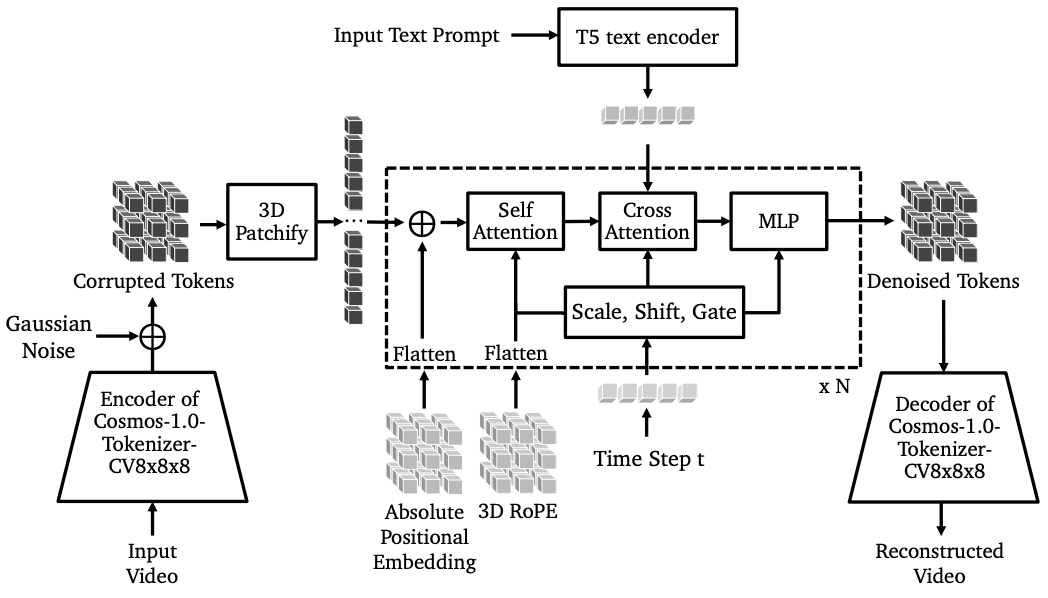
\includegraphics[width=1.0\textwidth]{./img/diffusion_arch.png}
            \end{center}
		\end{column}
		\begin{column}{.5\textwidth}
            \begin{center}
                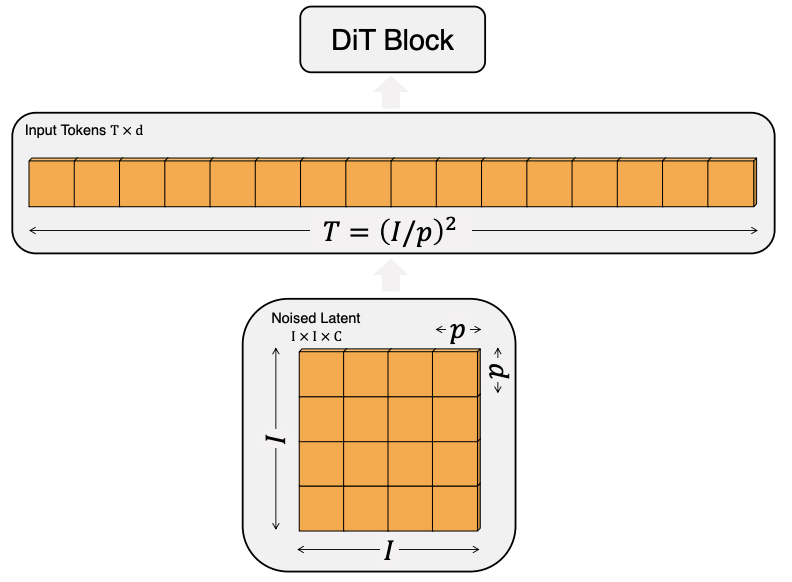
\includegraphics[width=1.0\textwidth]{./img/diff_arch_patch.png}
            \end{center}
		\end{column}
	\end{columns}
    % have video, run in through tokenizer, pertubate with gaussian noise
    \textbf{3D Patchification:}
    % DiT Process:
    % get latent rerpesentations throug heoncdoer - decoder 
    % diffusion happens in the latent space of the image
    \begin{itemize}[label=-]
        \item From tokenizer, input is latent representation $x \in R^{T \times C \times H \times W}$ 
        \item Downsample cubes of shape $p_t, p_h, p_w$ into individual input tokens via linear layer and flatten to 1D vector
        % patchification: have input I x I x C (after encoder) and then flatten each patch and flatten image and then mapped to a 
        \item image / videos reshaped to 1D, spatio temporal seq length $\frac{T H W}{p_t p_h p_w}$
        % \item use $p_t = 1, ,p_h=p_w=2$
    \end{itemize}
\end{frame}

\begin{frame}[t]{Architecture (positional encoding)}
    \vspace{-1.6em}
    \begin{center}
        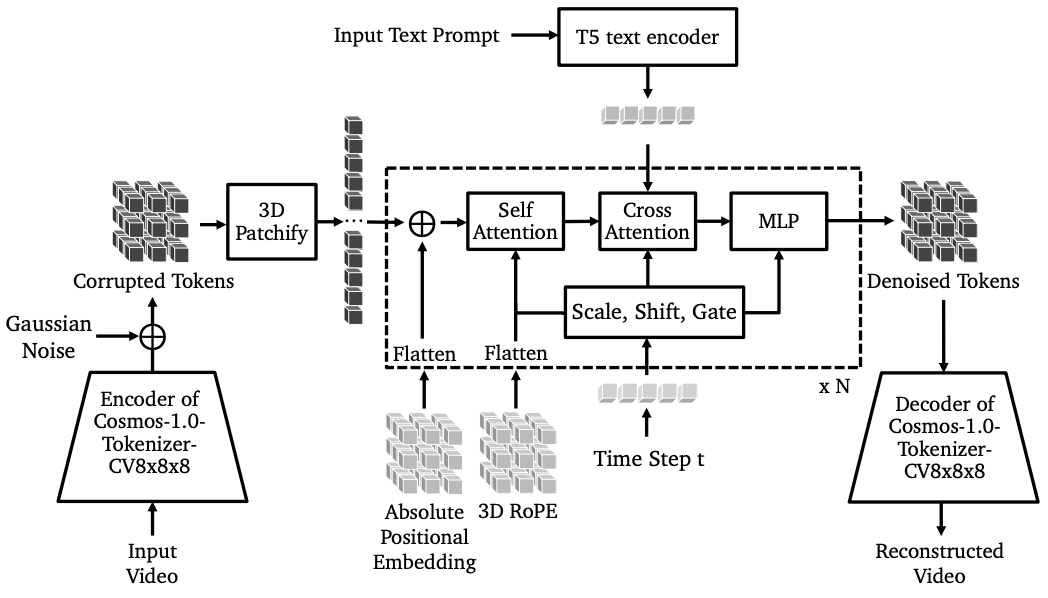
\includegraphics[width=0.7\textwidth]{./img/diffusion_arch.png}
    \end{center}
    % have video, run in through tokenizer, pertubate with gaussian noise
    % partition feature dim into 3 approx equal chunks, apply RoPE along temporral, height, width axes
    \begin{itemize}[label=-]
        \item partition feature dim into 3 approx equal chunks representing $T, W, H$, apply RoPE across each dimension
        % apply to the corresponding patches between splitting 
        \item Rescale temporal frequencies based on video FPS
        \item Add an absolute (learnable) positional embedding % increases perfrormance
   \end{itemize}
\end{frame}


\begin{frame}[t]{Architecture (Attention)}
    \vspace{-1.6em}
    \begin{center}
        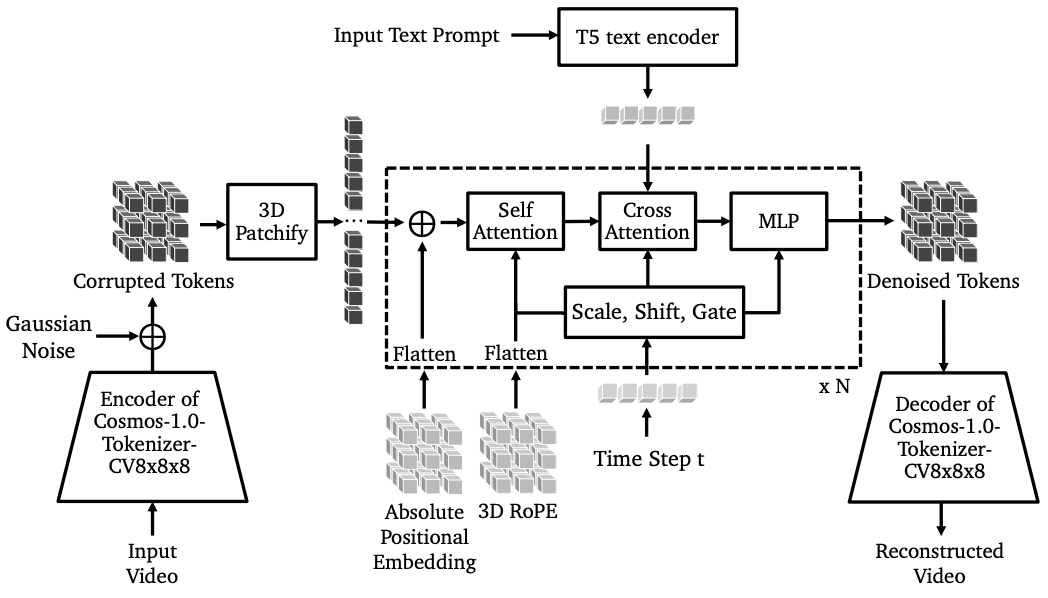
\includegraphics[width=0.7\textwidth]{./img/diffusion_arch.png}
    \end{center}
    \textbf{Cross Attention:} keys and querries from T5-XXL etext encoder\newline

    \textbf{Query-Key Normalization} before attention (RMSNorm) 
    % each transformer block is sequential self.attn, ccross-attn, and feed foward layers
    \begin{itemize}[label=-]
        \item  QK-norm applied before attn layers
        \item  fucus on re-scaling, ignore re-centering aspect of normalization
        \item Significantly reduce computation
        % apply RMSNorm normalization across hear of each query and key matrix priori to multiplying
        % only focus on re-scaling and ingoring the re-centering aspect or normalization
        % significantly reduct computation
        % then scale up by learnable parameter
   \end{itemize}
\end{frame}

\begin{frame}[t]{Conditioning Transformer Inputs}
    \vspace{-1.1em}
    How to condition transformer on time step $t$, class label $c$, prompt ...? \newline
	\begin{columns}[t]
		\begin{column}{.5\textwidth}
            \textbf{In-context Conditioning:}\newline
            Append embeddings of $t$ and $c$ as two additional tokens in input sequence.
            Remove them after final block.
            \textit{$\sim$0\% $\uparrow$ Gflops}.
            \newline
            \textbf{Cross-attention Block}\newline
            Create sequence of lenght 2: $[t,c]$. 
            Modify DiT block to have additional mha block
            \textit{15\% $\uparrow$ Gflops}.
		\end{column}
		\begin{column}{.5\textwidth}
            \begin{center}
                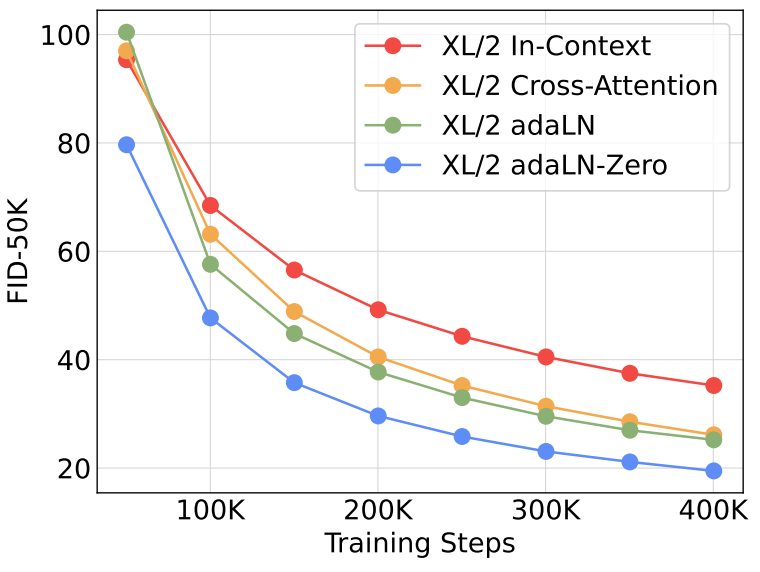
\includegraphics[width=1.0\textwidth]{./img/diff_arch_norm.png}
            \end{center}
		\end{column}
	\end{columns}
    Is there a more efficient way to achieve performace of cross-attn with less compute? \newline
    YES: \textbf{Adaptive Layer Normalization (AdaLN)} \newline
\end{frame}

\begin{frame}[t]{Conditioning Transformer Inputs}
    \vspace{-1em}
	\begin{columns}[t]
		\begin{column}{.5\textwidth}
            \textbf{Layer Norm:}
            \[\textbf{h} = \gamma \dot N(x) + \beta, N(x) = \frac{x - \mu}{\sigma}\]
            $\mu$ and $\sigma$ are mean and sd of $x$. $\gamma$ and $\beta$ are learnable vectors.

            \textbf{Adaptive Layer Normalization (AdaLN):} \newline
            Learn $\gamma$ and $\beta$ from sum of $t$ and $c$ embeddings.
            \[\gamma, \beta = \text{MLP}(t + c)\]
		\end{column}
		\begin{column}{.5\textwidth}
            \begin{center}
                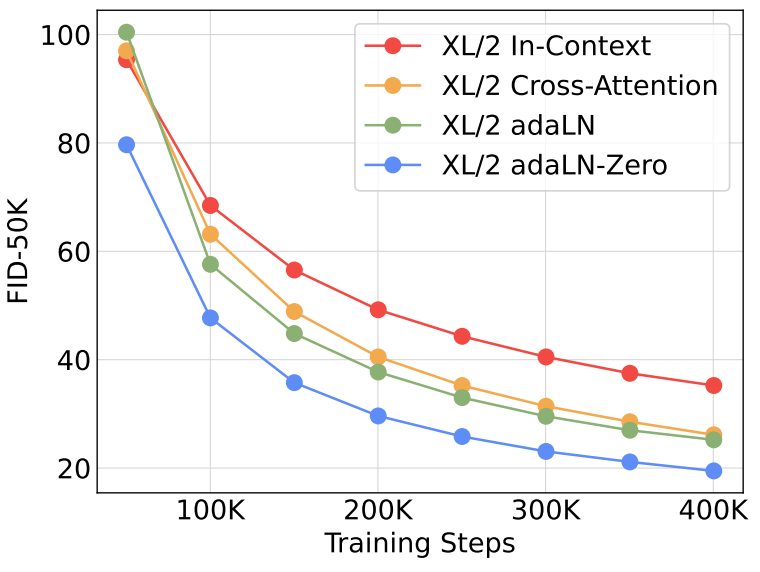
\includegraphics[width=1.0\textwidth]{./img/diff_arch_norm.png}
            \end{center}
		\end{column}
	\end{columns}
    \vspace{1em}


    
    % adaptive layer norm was propossed as a way of conditioning on external info
    % 
    \textbf{AdaLN-Zero:}
    Inspiration from initializing scalars (residual block as identity fn)
    \newline
    Compute $\alpha$ in addition to $\gamma$ and $\beta$ as scaling parameters.\newline
    $\alpha$ initialized as 0.
\end{frame}

\begin{frame}{DiT Block}
	\begin{center}
            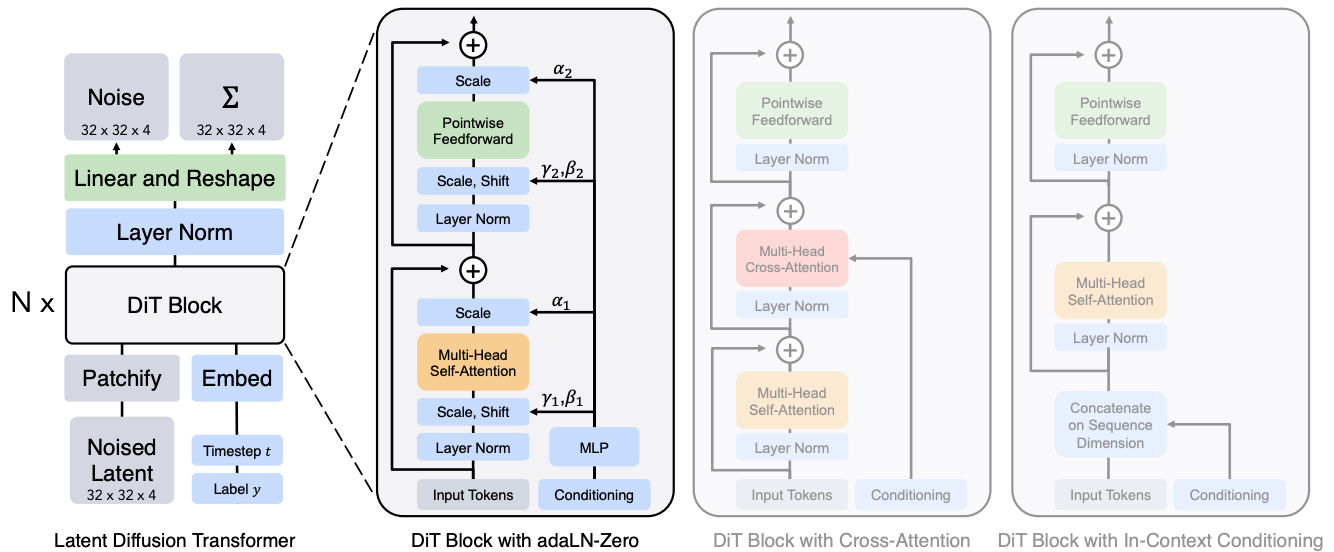
\includegraphics[width=1.0\textwidth]{./img/diff_arch_final.png}
	\end{center}
    \textbf{AdaLN-LoRA:}\newline
    % how possible since DiT claim they were efficient?
    Add LoRA to AdaLN layers, achieving 36\% reduction in parameter count, while maintaining performance.
\end{frame}

\begin{frame}{Training Details}
    % text2world: video generation model
    % video2world: video generation model conditioned on videos
    \textbf{Text2World}
    \begin{itemize}[label=-]
        \item Interleave batches of image and video data, scaling from 512p @ 57 frames to 720p @121 frames
        \item Organize data into 5 aspect ratios (1:1, 3:4,\dots), process frames from same bucket in each batch
        \item Two copies of model weights: BF16 for forward and backward pass. FP32 used for parameter updates.
        % iotroduce noise to conditional frames  to have more robust against generation mismatch
        % add a binary mask to distinguish f_c from f_g
        % exclude f_c from loss
   \end{itemize}
    \textbf{Video2World}
    \begin{itemize}[label=-]
        \item Image and Video conditioning by concat. conditional frames $f_i$ with generated frames $f_j$ along temporal dimension,
        introducing noise to $[f_i$: $f_1, f_2, g_1, g_2]$  
        \item binary mask concatonated along channel dimension to remove $f_i$ from loss calculation
   \end{itemize}
   \textbf{Prompt Upsampler:}\newline
   WFM use detailed video descriptions during training as text inputs. \newline 
   Finetune LLM to add detail to user prompts during inference
\end{frame}

\begin{frame}{Cosmos Results}
    30-second videos generated auto-regressively conditioned on first 9 frames. 
	\begin{center}
            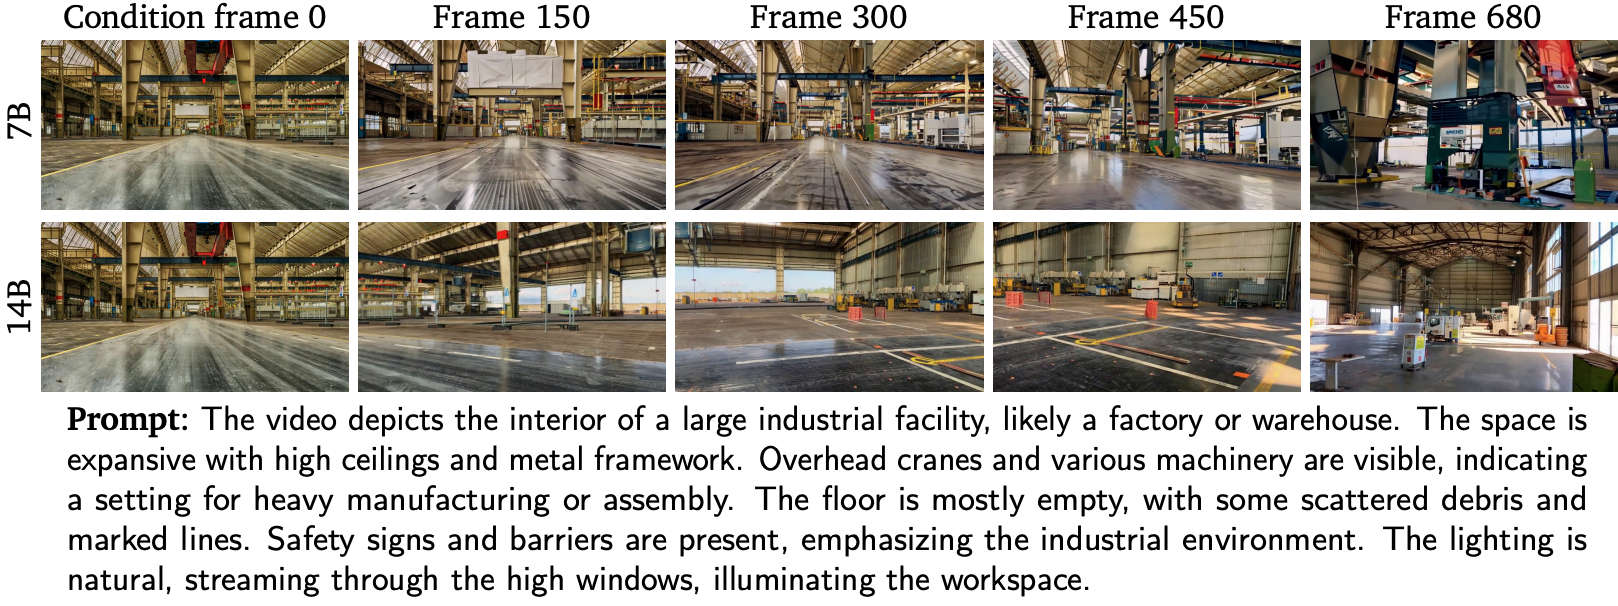
\includegraphics[width=1.0\textwidth]{./img/diff_arch_result.png}
	\end{center}
\end{frame}

\section{autoregressive-based WFM}
\begin{frame}{Formulation}
    World simulation generation as next-token prediction task (LLM style).\newline
    \vspace{-1em}
    \begin{enumerate}[label=\arabic*.]
        \item Tokenize video with cosmos tokenizer: $V = \left\{v_1, v_2, \dots, v_n \right\}$
        \item train to minimize: \[\mathcal{L}_{NLL} = \sum_i -log \pi_\Theta(v_i | v_1, v_2, \dots, v_{i-1})\]
    \end{enumerate}
\end{frame}

\begin{frame}{Architecture}
	\begin{center}
            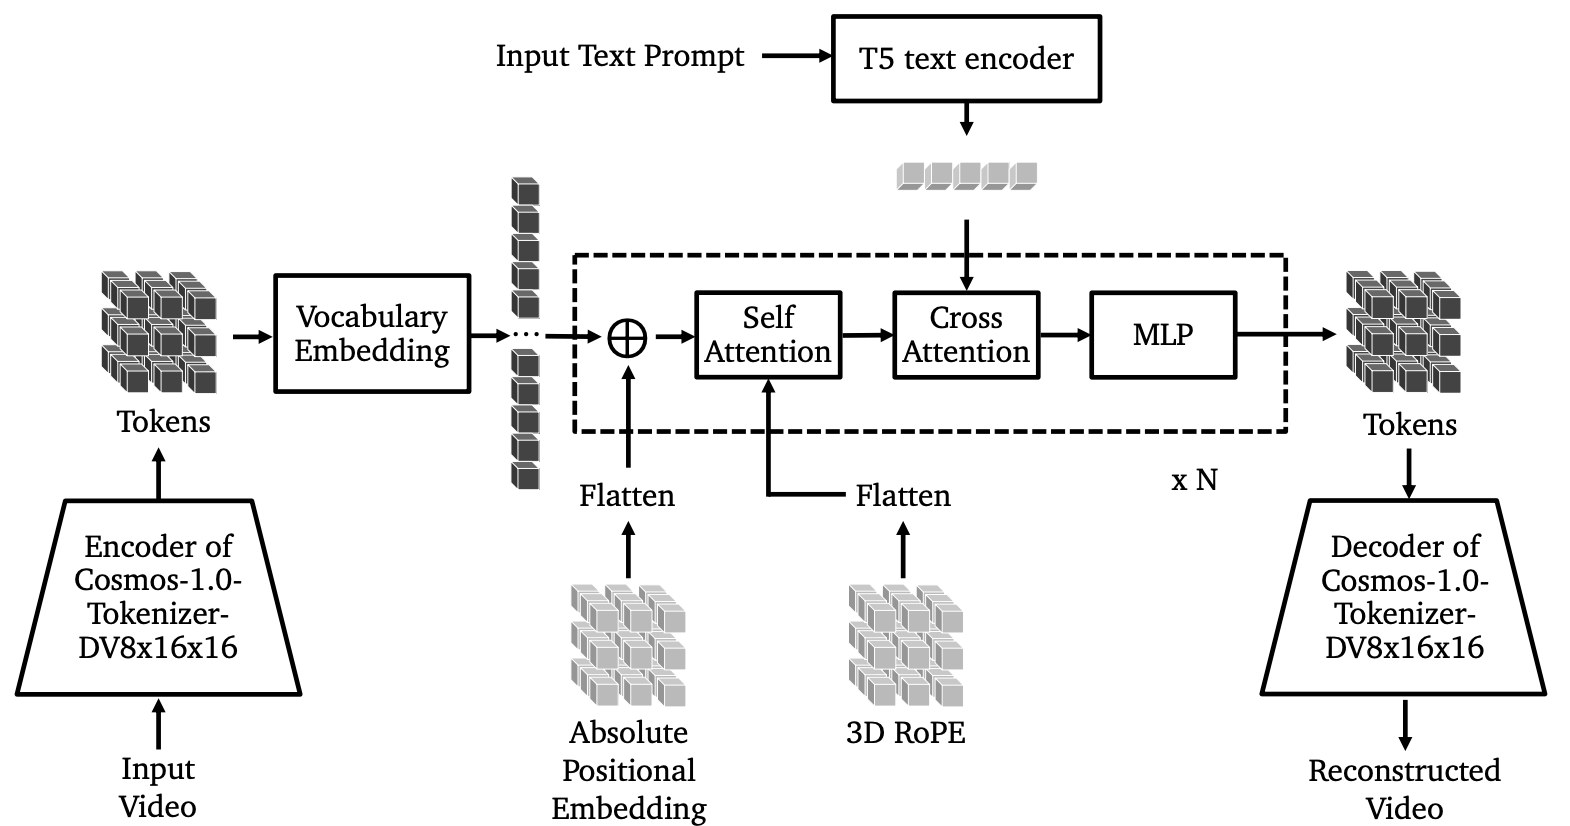
\includegraphics[width=0.8\textwidth]{./img/auto_arch.png}
	\end{center}
    \textbf{3D positional embeddings:} 3DRoPE and 3D Absolute Positional Embeddings 
    (sin and cos across temporal, ehight, width)\newline
    \textbf{Cross attention:} after every self-attn \newline

\end{frame}

\begin{frame}{Architecture}
	\begin{center}
            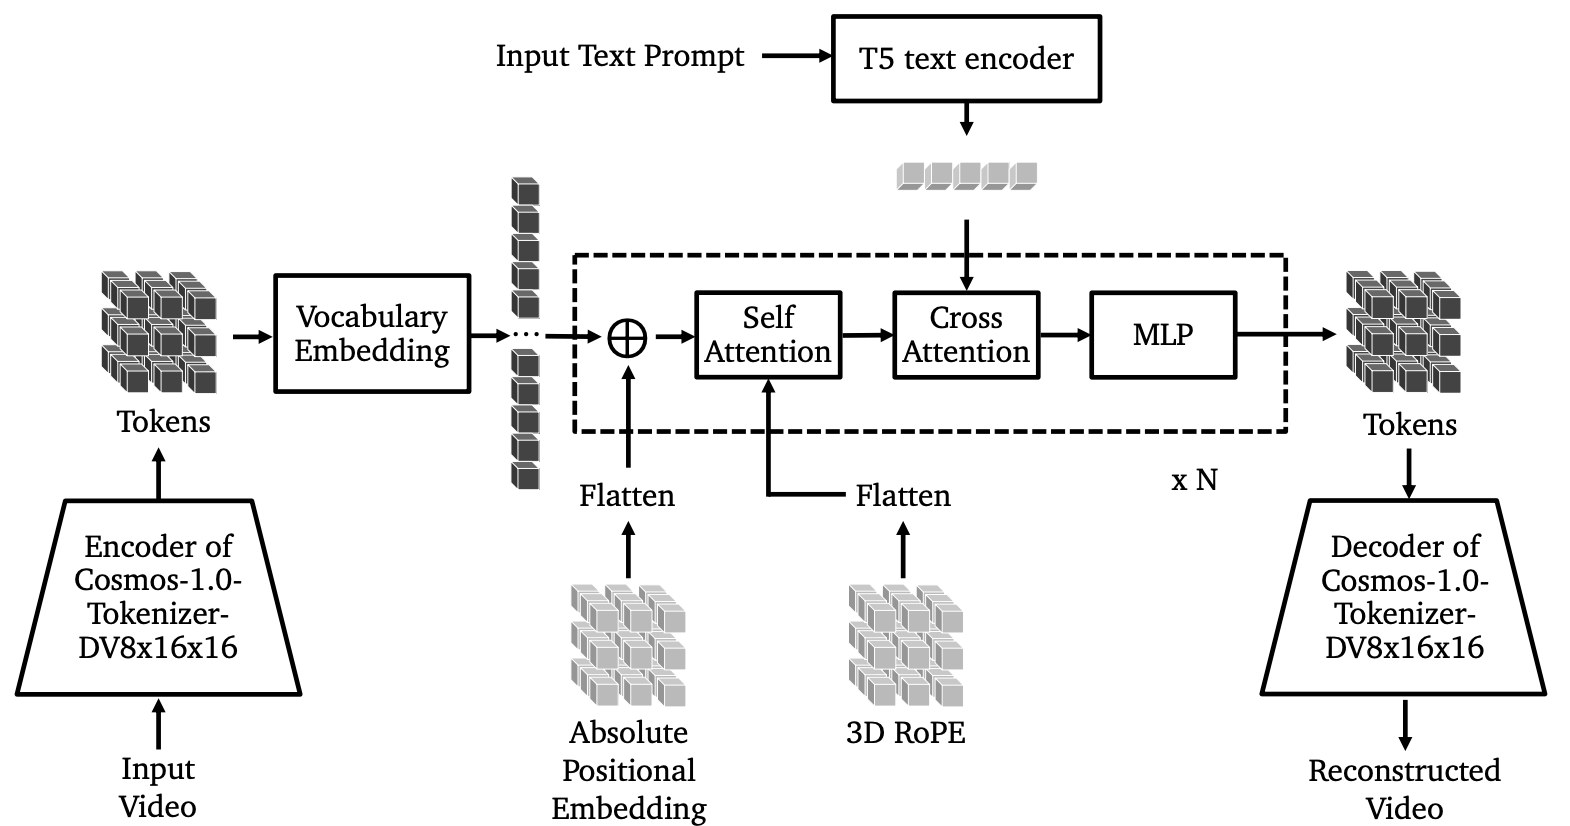
\includegraphics[width=0.6\textwidth]{./img/auto_arch.png}
	\end{center}
    \textbf{Query-Key Normalization (QKNorm):} 
    \begin{itemize}[label=-]
        \item Normalizes $Q$ and $K$ before computing dot product
        \item Dot product scaled by learnable param $\gamma$ instead of $\sqrt{d_k}$\newline
    \end{itemize}
    \textbf{Z-loss:} penalizes deviations of logics from 0
    % prevents generating large logit values bc give instability / gradient explosions
    \[\mathcal{L}_{\text{z-loss}} = \lambda \sum_i z_i^2\]

    % prevents softmax function from saturating and more efficient

\end{frame}

\begin{frame}{Training Details}
    \textbf{Pre-Training}:
    \begin{itemize}[label=-]
        \item \textbf{Stage 1:} Predict 16 future frames conditioned on first frame (context length = 17)
        \item \textbf{Stage 1.1:} Increase context length to 34 frames
        \item \textbf{Stage 2:} Text-conditioned generation with image-video batches similar to diffusion data 
    \end{itemize}
    \textbf{Cooling Down}: Linearly decay learning rate to 0 while training on high-quality image-vidoe pairs over 30k iterations.

\end{frame}

\begin{frame}{Diffusion Decoder (Training)}
    \textbf{Problem:} enc-dec tokenizer leads to blurriness, esp with discrete tokens \newline
    \textbf{Solution:} Diffusion decoder design.
	\begin{center}
            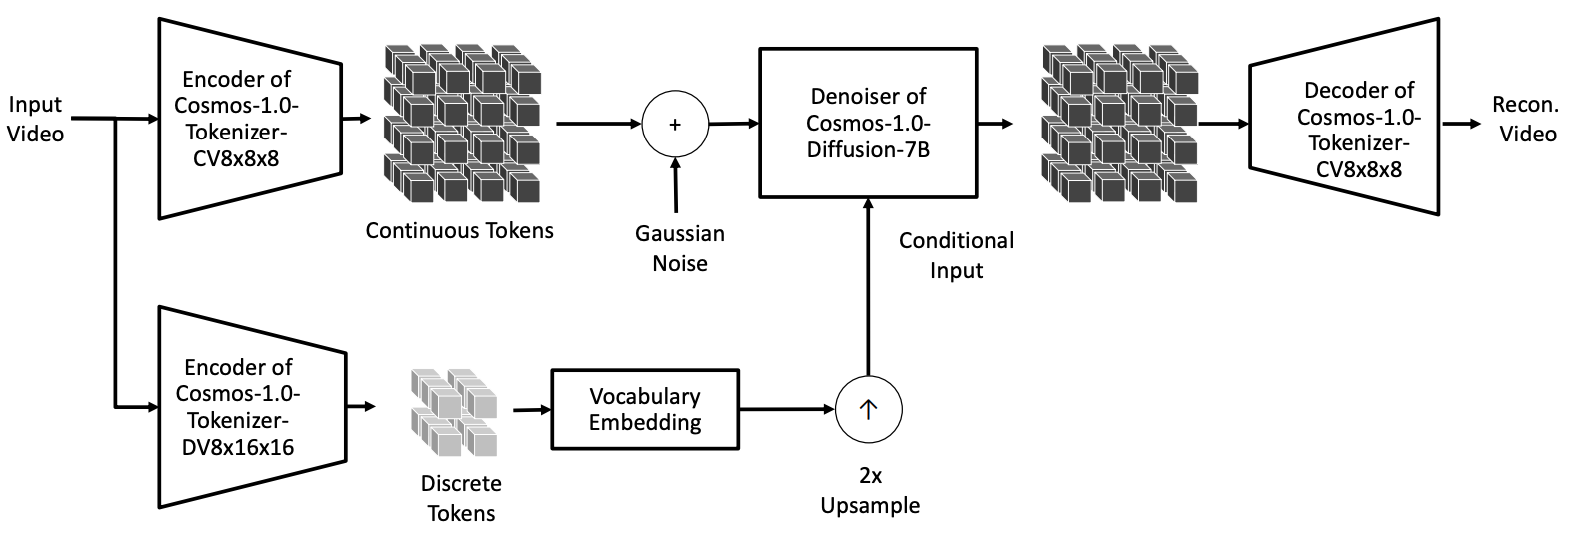
\includegraphics[width=1.0\textwidth]{./img/auto_decoder_arc.png}
	\end{center}
    % dimension of continuous tokenizer: 16 for each token
    % use less aggressive 8 x 8 x 8 (compression count scheme) than 8 x 16 x 16
    % embedd each discre token to 16-dim learnable vocabulary vector
    % more agressive compression scheme (2x more along x and y) so upsample to match cv
    % concatonate along channel dimension ( expand first dimension of tokenizer)
    \textbf{Result:} Higher-quality decoder that uses info in conditional input for denoising

    % tokenizer uses a enc-dec, lead to blurriness and artifacts generation
    % especially visible in discrete tokenization

    % 
\end{frame}

\begin{frame}{Diffusion Decoder (Inference)}
    During inference, video tokens conditionally inputed to decoder.
	\begin{center}
            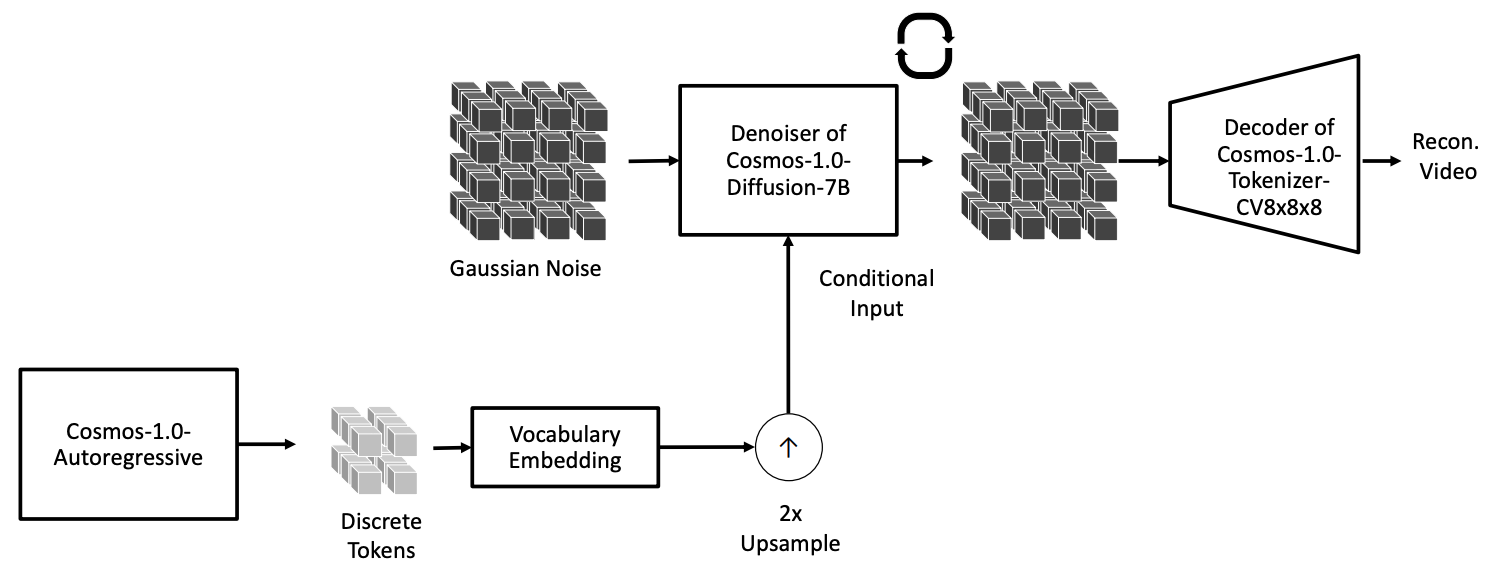
\includegraphics[width=1.0\textwidth]{./img/auto_arch_inf.png}
	\end{center}
\end{frame}

\begin{frame}{AutoRegressive Model Results}
    % better results anbd motion forom higher parameter count model
	\begin{center}
            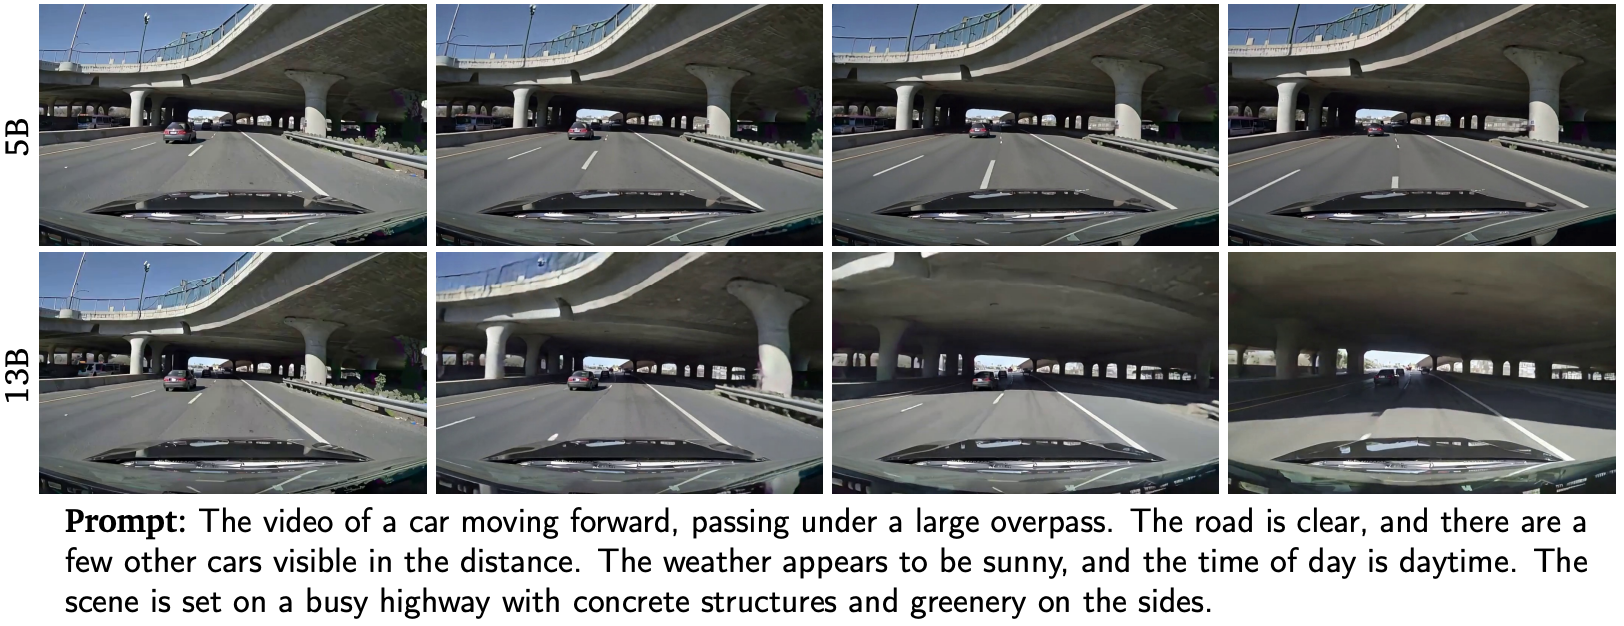
\includegraphics[width=1.0\textwidth]{./img/auto_arch_results.png}
	\end{center}
\end{frame}

\section{Post-Trained WFMs }
% paper  provided 3 examples of camera control, self-driving, and manipulation


\begin{frame}{Planner and Simulator Applications}
    \vspace{-1em}
	\begin{columns}[t]
		\begin{column}{.5\textwidth}
            \small
            \textbf{Instruction-based video prediction:}
            \begin{itemize}
                \item \textbf{Input:} current video frame, text instruction
                \item \textbf{Output:} video robot following instruction
            \end{itemize}
            \begin{center}
                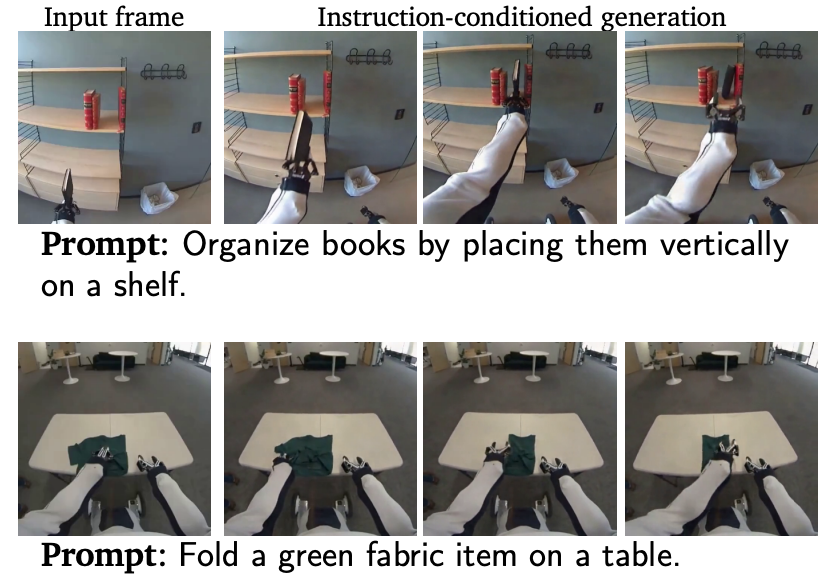
\includegraphics[width=1.0\textwidth]{./img/post_inst.png}
            \end{center}
		\end{column}
		\begin{column}{.5\textwidth}
            \small
            \textbf{Action-based next-frame prediction:}
            \begin{itemize}
                \item \textbf{Input:} current video frame, action vector
                % action vector between the current and next video fram
                \item \textbf{Output:} frame robot performing action 
            \end{itemize}
            \begin{center}
                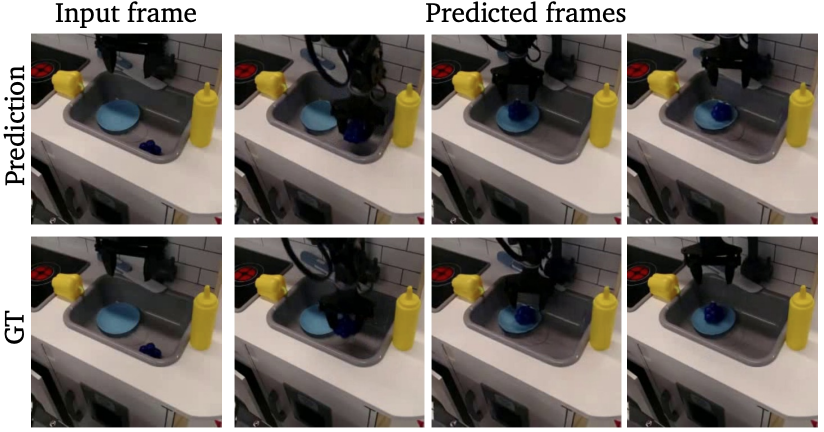
\includegraphics[width=1.0\textwidth]{./img/post_action.png}
            \end{center}
		\end{column}
	\end{columns}

\end{frame}

\begin{frame}{Datasets}
    \vspace{-1em}
	\begin{columns}[t]
		\begin{column}{.5\textwidth}
            \small
            \textbf{Instruction-based video prediction:}
            \begin{itemize}[label=-]
                \item Generate 200 hrs of EVE performing tasks
                \item Select 12k 1-9sec eposides
                \item Label actions, then upsample with VLM
                % tasks; naviga5tion, folding clothes
            \end{itemize}
		\end{column}
		\begin{column}{.5\textwidth}
            \small
            \textbf{Action-based next-frame prediction:}
            \begin{itemize}[label=-]
                \item Bridge dataset: 20k episodes at 5 FPS of 7-DOF arm performing tasks
                \item Each frame has action defined as 7-dim vector: \[\hspace{-1em}(\Delta x, \Delta y, \Delta z, \Delta \theta_r, \Delta \theta_p, \Delta \theta_y, \Delta_{\text{Gripper}})\]
            \end{itemize}
		\end{column}
	\end{columns}
    \begin{center}
        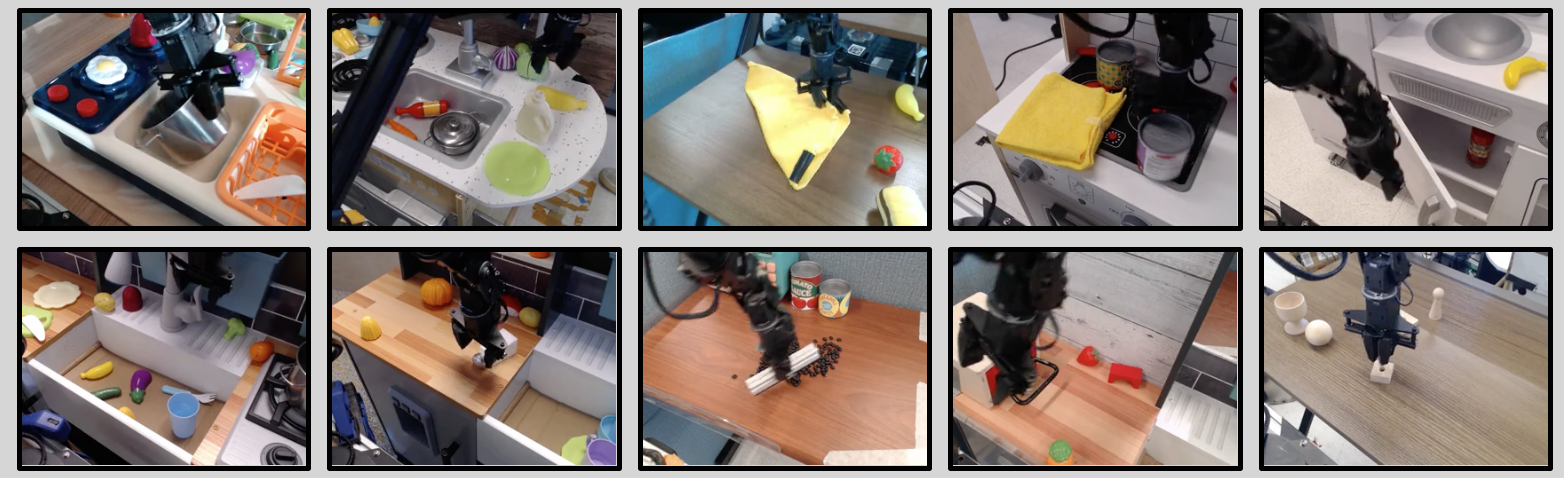
\includegraphics[width=0.9\textwidth]{./img/post_ds.png}
    \end{center}
\end{frame}

\begin{frame}{Fine-tuning and Evaluation}
    \vspace{-0.5em}
	\begin{columns}[t]
		\begin{column}{.5\textwidth}
            \small
            \textbf{Instruction-based video prediction:}
            \begin{itemize}[label=-]
                \item Compute T5 embeddings for instructions
                \item \textit{added via cross-attn}
                % tasks; naviga5tion, folding clothes
            \end{itemize}
		\end{column}
		\begin{column}{.5\textwidth}
            \small
            \textbf{Action-based next-frame prediction:}
            \begin{itemize}[label=-]
                % action new modality not seen during pre-training
                \item Add MLP to project action-vector to tensor
                \item \textit{added via cross-attn}
            \end{itemize}
		\end{column}
	\end{columns}
    \begin{center}
        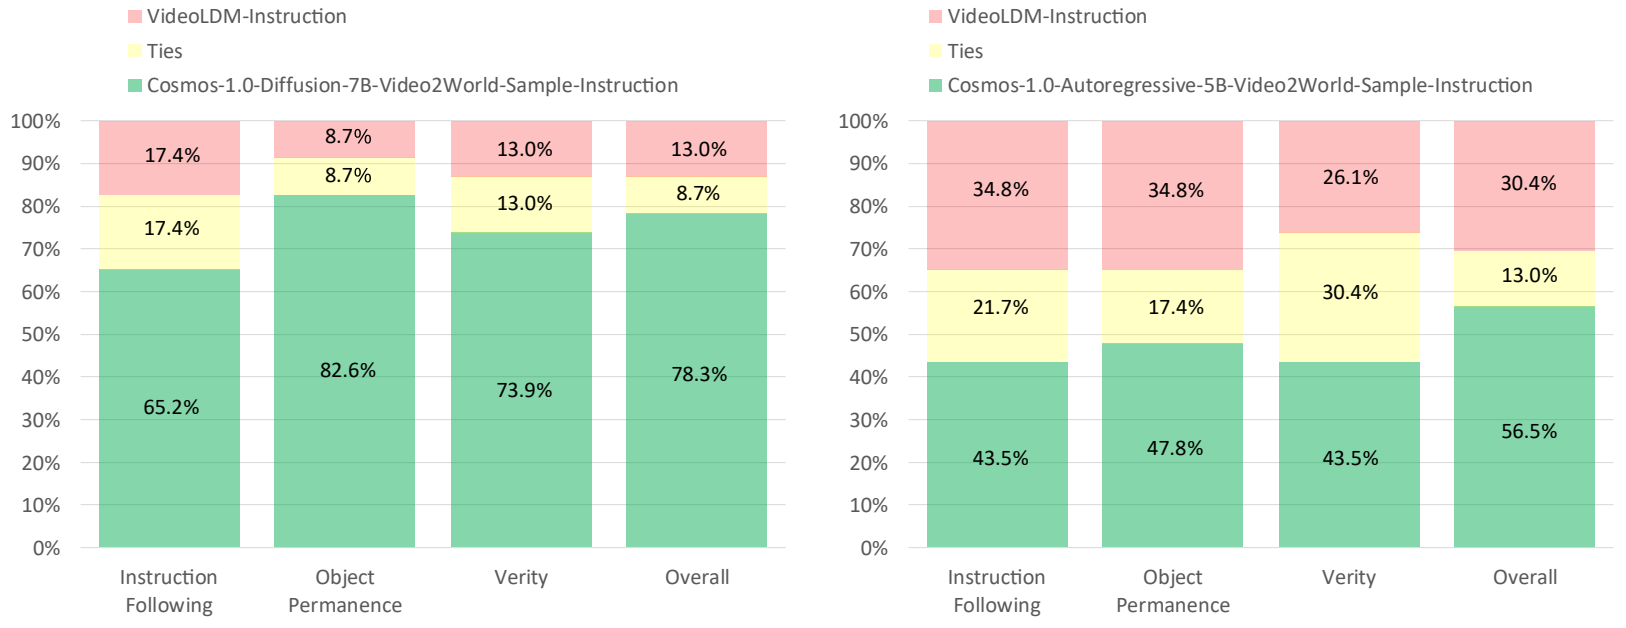
\includegraphics[width=0.8\textwidth]{./img/post_res_inst.png}
    \end{center}
    \begin{center}
        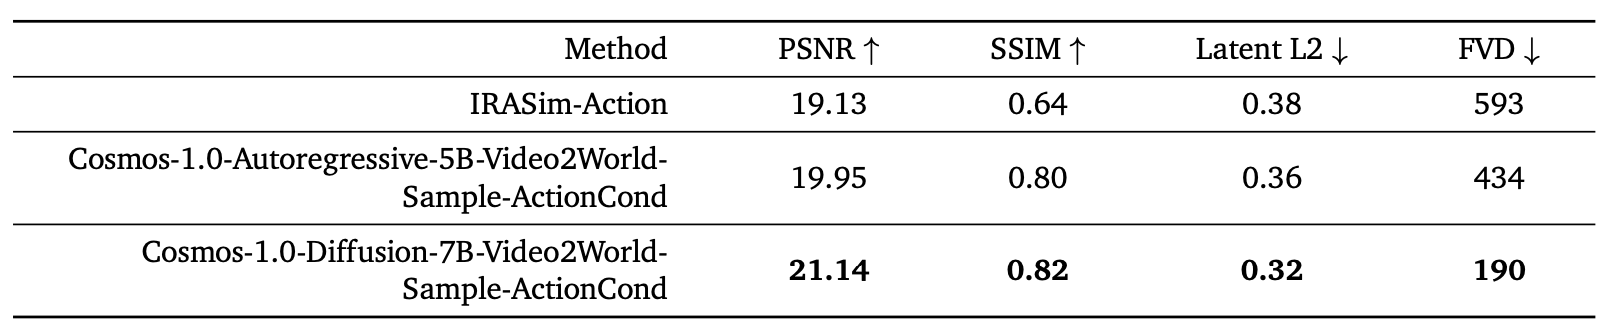
\includegraphics[width=0.8\textwidth]{./img/post_res_action.png}
    \end{center}
\end{frame}

\begin{frame}{Thank you!}
	\begin{center}
        Have a great rest of your Day!!!
	\end{center}
	\begin{center}
		% \textbf{Slides:} {\small \url{https://cs.purdue.edu/homes/jsetpal/slides/dnc_by_agop.pdf}}
	\end{center}
\end{frame}


\end{document}